\documentclass[]{article}
\usepackage{amsmath}
\usepackage{graphicx}
\graphicspath{ {.}}
%opening
\title{Algorithmic game theory HW0}
\author{Daniel Campos  \tt {dcampos3@illinois.edu}}
\date{09/01/2020}

\begin{document}

\maketitle

\section{Problem 1}
Let $a_1,a_2,...,a_n$ be fixed real numbers and $X$ be a random variable that takes value $a_i$ with a probability $p_i$. 
\subsection{Define the set of probability distributions that maximize $E[X]$}
\section{Problem 2}
Consider throwing $n$ balls into $n$ bins where each ball is thrown independently and uniformly into a bin
\subsection{What is the probability that a given bin(say the first bin) is empty}
\subsection{What is the probability that it contains exactly K balls}
\subsection{What is the expected number of bins that are empty}
\section{Problem 3}
Consider the following linear program \\

\begin{align}
max \; c^Tx \\
s.t \;\; Ax \leq b \\
x \geq 0
\end{align}

\subsection{Write the dual linear program of the above LP}
\subsection{Write the corresponding complementary slackness conditions}
\subsection{Using the complementary slackness conditions, derive the strong duality theorem}.(If $x^*$ is an optimal solution to the primal LP and $y^*$ is an optimal solution to the dual LP then $c^Tx^* = b^Ty^*)$
\section{Problem 4}
A wheel of size $k$ consists of a cycle on $k$ vertices along with an additional vertex connected to every vertex in the cycle. As an example, you can see with a wheel the size 8 in the figure below. \\
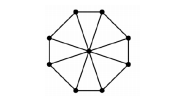
\includegraphics{8k}\\
The WHEEL problem is the
following
\subsection{Given an undirected graph $G = (V,E) $ and an integer $k$ does $G$ contain a wheel of size $k$ as a sub graph?}
\subsection{Prove that Wheel is NP-Complete}
reduce from Hamiltonian cycle problem
\end{document}
